\documentclass[11pt, a4paper, twocolumn]{jsarticle}
%
\usepackage{amsmath,amssymb}
\usepackage{bm}
\usepackage{graphicx}
\usepackage{ascmac}
\usepackage{subfigure}
\usepackage{multicol}
\usepackage{setspace}
\usepackage{mediabb}
\usepackage{float}
\usepackage{latexsym}
\usepackage{url}
\usepackage{cite}
%
\setlength{\textwidth}{\fullwidth}
\setlength{\textheight}{35\baselineskip}
\addtolength{\textheight}{\topskip}
\setlength{\voffset}{-0.5in}
\setlength{\headsep}{0.3in}
%
\renewcommand{\baselinestretch}{0.9}
\renewcommand{\figurename}{図}
\renewcommand{\tablename}{表}
\renewcommand{\headfont}{\bfseries}

\pagestyle{empty}

\begin{document}
% \twocolumn[
% \begin{screen}
% \begin{flushleft}
% aa\hspace{\fill}yyyy/mm/dd
% \end{flushleft}
% \begin{center}
% {\Large  和文タイトル  \\
% 英文タイトル}
% \end{center}
% \begin{flushleft}
% 工学系研究科 電気系工学専攻 関谷研究室\hspace{\fill}修士課程1年 37-136482 藤居 翔吾
% \end{flushleft}
% \end{screen}
% ]

\twocolumn[
\vspace{1.5cm}
\begin{center}
{\Large Multipath TCPを用いたデータセンターネットワークの改善}\\
\vspace{1em}
{\large $藤居\;翔吾^{\dagger}$ \hspace{1.0cm}$田崎\;創^{\ddagger}$ \hspace{1.0cm}
$関谷\;勇司^{\ddagger}$}\\
${}^{\dagger}$東京大学大学院工学系研究科\\
${}^{\ddagger}$東京大学情報基盤センター \\
\end{center}
\begin{quotation}
\begin{spacing}{0.6}
{\footnotesize クラウド型のサービスの性質により, 今日のデータセンターではデータセンター内のトラフィックが増大しており,
既存のTCPを拡張したMultipath TCP(MPTCP)により, 通信性能向上を目指す取り組みがされている.
しかし, 様々なニーズを抱えるトラフィックが混在している中で, レイテンシ志向なサイズの小さいフローに対し, MPTCPが性能を劣化させる問題が報告されている.
そこで本論文では, この問題に対し, 並列分散処理アプリケーションが稼働しているクラスターPCのトラフィックを観測する事で, 単一NIC(Network
Interface Card)への通信集中による遅延の影響がある事を示し, MPTCPによるデータセンターモデルのように複数のNICを持つノードが存在する環境で,
通信経路を切り替えることによりNICの負荷を分散させる手法を提案した.
この手法による効果について, 中継スイッチとエンドノードに対してスループット, フロー完結時間の二つのメトリックを用いた検証を行い,
改善手法が与える影響を考察する.
}
\end{spacing}
\end{quotation}

\begin{center}
{\Large Improving the datacenterr network with Multipath TCP }\\
\vspace{1em}
{\large ${\rm Shogo\;Fujii^{\dagger}}$
\hspace{1.0cm}${\rm Hajime\;Tazaki^{\ddagger}}$ \hspace{1.0cm}
${\rm Yuji\;Sekiya^{\ddagger}}$}\\
${}^{\dagger}$The University of Tokyo, Graduate School of Engineering\\
${}^{\ddagger}$The University of Tokyo, Information Technology
Center \\
\end{center}
\begin{quotation}
\begin{spacing}{0.6}
{\footnotesize
As increasing the amount of traffic in a datacenter by cloud service, the
effective network for utilization of massive computer clusters has been studied.
Recently, Multipath TCP(MPTCP) has been tackled this problem.
MPTCP can achieve the effective consumptions of the resources with multipath,
but a researcher reported MPTCP causes the delay of flow completion for short
flows.
In this paper, I presented measurements of the distribute processing cluster PCs
and reveal impairments that lead to that latencies, rooted in single NIC(Network
Interface Card) with intensive load traffic, and proposed the method balancing
the load for multiple NIC, in such a MPTCP datacenter model.
I verified the effect of the method for switch and end-node with two metrics,
FCT(Flow completion time) of short flows and throughput of backgroung flows,
and considered the effects of the load balancing.
}
\end{spacing}
\end{quotation}

\vspace{1.5cm}
]


\section{導入}


今日の一般家庭のインターネット接続環境がギガビット級の速度に達しようとしている中, 多様の端末がインターネットに接続できるようになり,
大量かつ多種多様なデータの取得が可能となった.
特にトラフィックデータ量の増加傾向は顕著で, 18$\sim$24ヶ月単位で総データ容量が2倍になるという予測がされている~\cite{IBM_rep}.
またFacebookでは, 300ペタバイト以上のデータ量を保有しており, 1日あたりに1ペタバイトのデータを解析している~\cite{presto}.
このように近年では, ビッグデータの活用が着目され, 例えばウェブ検索エンジン, SNS(Social Networking
Service)などのデータセンターを用いたクラウド型サービスにおいて, リアルタイムに近いレスポンスを返すような場面で使われ始めている.
そのようなクラウドサービスには近年, より高いユーザーエクスペリエンスが要求されており,
Amazonでは100[ms]の遅延により売り上げが1\%下がる, といった報告~\cite{amazon}があるように,
例えばeコマースサイトでの商品購入や,
インターネット広告のコンバージョンのようなユーザの意思決定へのレスポンス遅延の影響は深刻な問題である~\cite{customer_impact}.
そのため, 大規模データをより高速に処理することが求められており, データセンターではサーバ運用台数が増加の一途を辿っている.
そうした中で, 可用性, 計算性能, 低コストの三つの要件がデータセンターの抱える課題となっている~\cite{requirement}.
特に計算性能について, 大量の計算機資源から最大限の性能を引き出すためには,
従来の仕組みではデータセンター内トラフィックに対して一部の資源にトラフィックが集中する問題に対応できないため,
計算機資源を有効活用するための研究が盛んに行われている\cite{mapreduce, dryad, fattree, bcube, vl2,
dctcp, improving, detail, p_fab}.
そのようなスケーラビリティ拡大には, ネットワークトポロジー, アプリケーション, プロトコルに対する三つのアプローチがある.

ネットワークトポロジーを改良するアプローチでは, 従来の単純な階層構造では,
データセンター内で発生するトラフィックに対して帯域が最大限割り当てられない~\cite{fattree}.
そのため, 近年ではそのようなトラフィックに対してスイッチを多段に構成することで帯域を有効利用するトポロジーが提案されている~\cite{fattree,
bcube, vl2}.

大量データの処理速度を改良するアプローチでは,
並列分散処理のためにpartition-aggregate計算モデルが提案されている.
MapReduce~\cite{mapreduce}, Dryad~\cite{dryad}等の並列分散処理フレームワークは,
この計算モデルに従っており, 今日の大規模クラウドサービスにおいては, 必要不可欠である.

プロトコルを改良するアプローチでは,
従来のTCPを拡張したMultipath TCP
(MPTCP)~\cite{mptcp}をデータセンターネットワークに用いる提案がされている~\cite{fattree,bcube,vl2}.
MPTCPを用いることにより, OSの制御によって複数のNIC(Network Interface Card), 複数の経路を同時に利用し,
スループットを向上させることが期待されている.

しかし, 並列分散処理フレームワークを用いることで, フローサイズの小さい大量のクエリーが発生し, MPTCPは,
フローサイズの小さいトラフィック(ショートフロー)に対しては, TCPよりも性能が劣化する問題が報告された~\cite{improving}.

このような背景から, 大規模データセンターネットワークへのMPTCP適用時のショートフロー遅延の問題は並列分散処理アプリケーションの性能の面で深刻な問題である.
そこで本論文では, データセンターにおけるショートフロー遅延の問題を解決する為に, 二つの検証を行った.

一つは, 実環境の並列分散処理アプリケーションが稼働しているクラスターPCを用いて, 実トラフィックの観測, 解析を行った.
クラスターPCがジョブを実行していない定常状態時と並列分散処理を実行している時の二種類のトラフィックを解析することで,
並列分散処理アプリケーションが生成するトラフィックパターンの特徴および, 汎用的なネットワーク機器を用いた低コストなデータセンターにおける要求案件を検証した.
そして, ショートフロー遅延が生じる状況と既存のネットワーク設計の背景について, ボトルネックとなりうるネットワーク環境を検討し, その原因を示した.

二つ目は, MPTCPを用いたデータセンターネットワークモデルにおける, 複数のNIC, 複数の経路を利用した経路切り替えによる改善手法を提案する.
これは, 複数の経路を利用し, スイッチやエンドノードの持つ複数のNICへと負荷を分散させることで, 単一のNICに負荷が集中することにより,
キューイングやプロトコル処理の遅延を抑える事ができる, という仮定に基づいた提案手法である.
この手法により, 並列分散処理におけるショートフローのように, 低レイテンシが求められる通信においては, 他のフローの影響を受けずにすぐに割込み処理が行われ,
受信処理のCPU負荷の分散を期待しており, その効果をシミュレーション, 実環境での実験を用いて検証した.
そして今後の課題として, 経路切り替えのアルゴリズム検討する.

% 本稿では, \ref{sec:related}章でMPTCPによるデータセンターネットワークモデルに関する先行研究を示し,
% \ref{sec:mptcp}章ではMPTCPの詳細を述べる.
% \ref{sec:fattree}章では近年提案されたネットワークトポロジーを紹介し, \ref{sec:traffic_scenario}章では
% データセンター内のトラフィックに関する特性を示す.
% そして, \ref{sec:reproduction}章では報告された問題を検証し,
% \ref{sec:evaluation}章ではデータセンターネットワークでのMPTCPの性能について評価, 考察する.
% 最後に, \ref{sec:conclude}章で本稿での検証結果についてまとめる.

\section{関連研究}
\label{sec:related}
本章では, これまでに報告されている複数経路利用によるフロー完結時間短縮化技術について簡潔に述べ, その優位性や問題点を示す.

2010年にAlizadehらによって, データセンターネットワーク特有のトラフィックパターンに特化して,
パラメータを決定するアルゴリズムが提案された~\cite{dctcp}.
データセンター特有のバースト性のあるトラフィックが引き起こす問題点として, キューの生成によるキューイング遅延, キュー溢れによるパケットロス,
スイッチのバッファに掛かる負荷がある.
これらの問題に対し, 経由するスイッチにおいて, ECN(Explicit Congestion Notification)によってエンドノードに輻輳を通知し,
キューの大部分が占有される前にウィンドウサイズを動的に変化させ, キューサイズを小さく保つアルゴリズムによって,
大部分のキューの伝送時間を短縮することを可能にした.
しかし, 大規模計算資源を想定したトポロジーにおける検証がされておらず, また各ネットワークデバイスに細かなチューニングを必要とするため,
大規模データセンターでは運用面での問題がある.
さらに, サイズの大きいフローの割合の大きいトラフィックの中では, その影響によりウィンドウサイズを小さくする制御が働くため,
サイズの小さいフローの完結時間への効果が小さい, と報告されている~\cite{p_fab}.

2011年にCostinらによって, MPTCPを用いたデータセンターネットワークモデルが提案された~\cite{improving}.
近年の大規模計算資源を有効活用するために提案されたネットワークトポロジーでは,
高性能なデバイスや特殊な機器を必要とせず, 汎用的なネットワーク機器のみを用いてデータセンター内のエンドノード同士の通信に経路が複数用意されている.
既存の取り組みでは, 通信に使わない経路をセカンダリ経路として利用することで, 耐障害性を持たせていたのに対し, 提案されたデータセンターモデルでは,
MPTCPを用い複数経路を同時に利用する事で, 耐障害性を保ちながら, 帯域を最大限利用する事を可能にした.
また, 様々なトポロジーにMPTCPを適用することで, 従来のTCPよりも高いスループットが出せることを示した.
しかし, MPTCPとSingle path-TCPが混在する環境において, Single
path-TCPで行われるサイズの小さいフロー($\leq70KB$)のフロー完結時間に着目すると, 従来のSingle
path-TCPのみのネットワーク環境よりも時間がかかるという問題点があった.

2012年にZarsらによって, 複数レイヤー間でトラフィックを監視し,
しきい値を設定することによるフロー完結時間の短縮化技術を提案した~\cite{detail}.
今日のデータセンター内ネットワークのような, サイズの異なるフローが混在するネットワークにおいては, サイズが小さいフローがサイズの大きいフローに圧迫され,
伝送遅延が大きくなる問題があったが, この提案手法では, データリンク層からアプリケーション層までの各層が,
相互にトラフィックを監視する機能をスイッチに実装し, 優先度をつけ, バッファサイズを調整することで, フロー完結時間の劣化を抑えることを可能にした.
しかし, 実験ではClick~\cite{click}を用いて実装を行っており, 現実世界での全てのネットワーク機器の置き換えが必要となるので, 実現は難しい.

以上で述べたことをまとめると, 近年のデータセンターネットワークに対して, 以下のような要件が考えられる.
\begin{itemize}
  \item 大規模計算機を有効活用するトポロジーの利用
  \item 分散処理の際に発生する大量のサイズの小さいフローの送信時間の短縮
  \item 特殊な実装やデバイスを用いず, シームレスな運用の実現
\end{itemize}

\section{データセンターネットワーク}
\label{sec:datacenter}
本章では, データセンターネットワークを構成する技術に関して, その概要を述べる.
\subsection{Multipath TCP}
MPTCPは, 一つの経路でデータ転送するTCPを拡張し, 複数のインタフェース,
複数のポートを用いてデータ転送をするプロトコルである~\cite{mptcp}.
クライアントが複数のIPアドレスを持っていた場合, 新たにサブフロー\footnote{複数のTCPコネクションの内,
ある一つのコネクションにおけるフロー}のコネクションが確立される.
追加されたサブフローは, インターフェース毎に異なるIPアドレスの組み合わせで通信を行う.
ルーティングに関しては, 複数の宛先, 送信元IPアドレスのペアからそれぞれ経路決定される.
このように, アプリケーション層より下のレイヤーのみで複数の経路を使ってデータ転送を行うため,
アプリケーション側がMPTCPでの通信を意識することなくデータ転送ができる.

さらにMPTCPでは, TCPと同様にAIMD(additive-increase and
multiplicative-decrease)による輻輳制御がサブフロー単位で行われ, 経路状態に合わせて輻輳制御をする~\cite{cong}.

% このアルゴリズムには, TCPと同様にAIMD(additive-increase and
% multiplicative-decrease)による輻輳制御がサブフロー単位で行われる.
% 以下にAIMDアルゴリズムを示す.
%
% \begin{itemize}
% \item サブフロー $r$において,
% 1ACKごとにウィンドウサイズ$\omega_{r}$をmin$(\frac{\alpha}{\omega_{total}},
% \frac{1}{\omega_r})$増加させる.
% \item サブフロー $r$において, パケットロス時にウィンドウサイズ$\omega_r$を$\frac{\omega_r}{2}$へ減少させる.
% \end{itemize}
% ここで, $\omega_{total}$は全てのサブフローのウィンドウサイズの総和, $\alpha$は送信速度の増加量を示すパラメータで,
% 以下のように定義される~\cite{cong}.
%
% \vspace{-2mm}
% \begin{eqnarray}
%  \alpha = \omega_{total} \times
% \frac{\displaystyle \max_{r} \frac{w_r}{RTT^2_r}}{\displaystyle
% (\sum_{r}\frac{w_r}{RTT_r})^2}
% \label{alpha}
% \vspace{-2mm}
% \end{eqnarray}
%
% ここで, $RTT_r$はサブフロー$r$でのラウンドトリップ時間を示している.
% MPTCPでの輻輳制御には二つの性質ある.
% 一つは, サブフローのウィンドウサイズは, 全てのウィンドウサイズの大きさに依存するということである.
% これにより, 混雑したサブリンクにおいては, ウィンドウサイズが抑えられ, ロードバランスができる.
% 二つ目は, MPTCPのアルゴリズムによって, TCPでの輻輳制御よりも悪化する事を回避している事である.
% しかし, もし複数のサブフローがそれぞれ混雑のないサブリンクを利用する場合, いずれかのコネクションが帯域を占有する可能性がある.

\subsection{FatTreeトポロジーとMPTCPによるデータセンターモデル}
\label{sec:fattree}
この節では, データセンターを構成する要素について述べる.
\subsubsection{トポロジー}
\label{subsec:topology}
従来のデータセンターモデルでは, HostがEdgeスイッチにつながり,
これらのスイッチがAggregationスイッチに集約され,
coreスイッチに接続するといったように, 階層的に二分木トポロジーを形成していた~\cite{fattree}.
このような単純な階層構造を持つトポロジーは, トラフィックの大部分がデータセンター外の通信には有効であった.
しかし, 今日のようなデータセンター内で生じるトラフィックが大半を占める場合, 上の階層にある広帯域の経路を使わない通信が増え, 帯域の割当が不適切である.
このような, データセンター内のトラフィックが主であれば, 階層型のトポロジーはボトルネックを引き起こす可能性がある.
近年の研究~\cite{fattree,bcube,vl2}では, トラフィックがデータセンター内に集中した時の問題を, 物理的なアプローチとして,
トポロジーを工夫する事で解消を試みている.

図\ref{fig:fattree}のように, FatTree~\cite{fattree}では, Coreスイッチを複数用いる事で,
物理パスの最大帯域を供給する.
また, 比較的狭い帯域の経路と汎用的な性能のスイッチを多数用い, データセンター内のエンドノード同士の通信で複数の経路を実現する事で, 冗長化,
ネットワーク資源の効率的な利用, 低コストを実現している.

しかしこのような密な配置により, 複数の経路が形成され, ルーティングをどのように決定すべきかという問題も生じる事となる~\cite{improving}.
例えば図\ref{fig:fattree}のようなFatTreeトポロジーでは, 4通りの経路が考えられる.
これら複数の経路をリンクエラー時の冗長性を持たせる目的だけでなく, 性能向上に活用することが求められている.
\begin{figure}[h]
    \begin{center}
    \includegraphics[autoebb, width=195pt]{./img/fattree_topology.pdf}
    \caption{Fattree トポロジー}
    \label{fig:fattree}
    \end{center}
\end{figure}
% \begin{figure}[h]
%     \begin{center}
%     \includegraphics[autoebb, width=180pt]{./img/hierarchy_topology.pdf}
%     \caption{階層型ネットワークトポロジー}
%     \caption{Hierarchical network topology}
%     \label{fig:hierarchical}
%     \end{center}
% \end{figure}

% \begin{figure}[h]
% \begin{minipage}{0.5\hsize}
% \begin{center}
% \includegraphics[autoebb, width=110pt]{./img/fattree_topology.pdf}
% \end{center}
% \caption{FatTreeトポロジー}
% \caption{Fattree topology}
% \label{fig:fattree}
% \end{minipage}
% \begin{minipage}{0.5\hsize}
% \begin{center}
% \includegraphics[autoebb, width=110pt]{./img/bcube.pdf}
% \end{center}
% \caption{BCubeトポロジー}
% \caption{BCube topology}
% \label{fig:bcube}
% \end{minipage}
% \end{figure}



% \section{再現シミュレーション実験}
% \label{sec:reproduction}
% この章では,
% Raiciuらによって示したFatTree-MPTCPネットワークモデルでのフローサイズの小さいトラフィックに対する性能評価シミュレーションを再現し,
% 解析を行った結果を示す.
%
% \subsection{再現シミュレーション実験環境}
% Raiciuらは~\cite{improving}において, 各プロトコルがフローサイズの小さなトラフィックに対して及ぼす影響の評価を行い,
% フローサイズの小さいトラフィックに関しては, MPTCPによりフロー完結時間を遅延させることを示した.
% そのときのシミュレーション環境は, 以下の通りである.
% ネットワークトポロジーには, 4:1にオーバーサブスクリプションされたFatTreeを用いている.
% ベンチマークトラフィックについては, ホスト同士の1対1通信を用いている.
% 全てのホストのうち, 33\%をTCPまたはMPTCPにより継続してデータ転送 (Background traffic)を行う.
% 残りのhostを使って, TCPによる70Kbyteのデータ転送(Short flow)を毎200[ms]のポアソン生起させ,
% 転送完了までにがかかった時間FCT(Flow Completion Time)を計測している.
%
% 今回の再現実験にはns-3 Direct Code Execution~\cite{ns3}を用い, MPTCPは, Linux
% カーネルソースを用いた~\cite{mptcp_linux}.
% 図\ref{fig:fattree_rep}に, シミュレーションで用いたFatTree(k=2)トポロジーを示す.
% このトポロジーでの物理パスでは, 一つのサブフローが1本の物理パスを占有するように, 設計している.
% すなわち, 4つのサブフローを使う場合, ホストの4インターフェースに対しそれぞれ4つIPアドレスが割り当てられる.
% また, Host-Edge部分には, IPアドレスの数だけインターフェースを用意し, Aggregation-Edge部分も,
% それに従いインターフェースを追加する.
% さらにルーティングに関しては, Core1$\sim$Core4に分散するようにルーティングテーブルを設定した.
%
% 表\ref{table:testbed}に再現シミュレーション環境に対する各パラメータをまとめる.
% \begin{table}[h]
% \begin{center}
% \footnotesize
% \begin{tabular}{c|c}
% \hline
% Parameter & Value \\ \hline \hline
% Nodes & 16 \\
% MPTCP & v0.88 \\
% Link core-aggr & 400Mbps \\
% Link aggr-edge & 200Mbps \\
% Link edge-host & 100Mbps \\
% RTT & 0.5ms\\
% Receive buffer size & 100KB \\
% \hline
% \end{tabular}
% \caption{Testbed on network simulation}
% \label{table:testbed}
% \end{center}
% \end{table}
%
% \begin{figure}[h]
%     \begin{center}
%     \includegraphics[autoebb, width=210pt]{./img/fattree_rep.pdf}
%     \caption{Network topology on reproducing simulation}
%     \label{fig:fattree_rep}
%     \end{center}
% \end{figure}
%
% \subsubsection{設定パラメータに対する有効性の検証}
% 伝搬遅延についてはRTT(Round Trip Time)として, 0.5[ms]に設定した.
% これは, 一般的なデータセンター内のRTTが1[ms]以下であるためである~\cite{rtt}.
%
% バッファサイズについては, 以下の帯域幅遅延積(BDP)の式から, 400Mbps$\times$4を最大限利用できるだけの値を設定した.
% \vspace{-2mm}
% \begin{eqnarray}
% BDP[{\rm byte}] = 帯域幅[{\rm bps}] \times RTT \div 8
% \label{cong}
% \vspace{-2mm}
% \end{eqnarray}
%
% 各帯域については, 16のノードを使って輻輳を引き起こす現象を再現するために, 実際のデータセンターのような広帯域のネットワークと比べ,
% 狭い帯域を設定した.
%
% \subsection{再現結果}
% 図\ref{fig:short_flow_rep}, 表\ref{table:short_flow_rep}に, 上記の実験環境で再現した結果を示す.
% 再現結果から, フローの様子を完結時間別に4パターンに分類することができることが分かった.
% 表\ref{table:flow_pattern}にそのフローパターンの定義を示す.
%
%
% 今回の再現実験において, TCPとMPTCPでフロー完結時間に差を生じた要因は, パケットロスが発生する割合にある.
% 図\ref{fig:cdf}に再現実験でのフロー完結時間ごとの累積確率分布を示す.
% パケットロスを生じないフローに関しては, 両者に性能差を感じなかったが, この図から, MPTCPを用いた方が,
% パケットロスを引き起こし遅延を生じさせる割合が大きいということが分かる.
%
% このようにMPTCPが帯域を大きく占有することにより他のトラフィックを圧迫することは, MPTCPの輻輳制御によるものだと考えられる.
% 混雑のない経路でデータ転送する場合, MPTCPでは積極的にウィンドウサイズを増やそうとするため, 他のフローに対し遅延を引き起こしたと推測される.
%
% \begin{figure}[h]
%     \begin{center}
%     \includegraphics[autoebb, width=210pt]{./img/flow_comp.pdf}
%     \caption{The result of the reproduction experiment}
%     \label{fig:short_flow_rep}
%     \end{center}
% \end{figure}
%
% \begin{figure}[h]
%     \begin{center}
%     \includegraphics[autoebb, width=210pt]{./img/cdf_rep.pdf}
%     \caption{CDF of flow completion time on reproduction experiment}
%     \label{fig:cdf}
%     \end{center}
% \end{figure}
%
% \begin{table}[h]
% \begin{center}
% \footnotesize
% \begin{tabular}{c|p{5em}|p{4em}|p{5em}}
% \hline
% Protocol & AVG comp time[ms]& Stdev[ms] &
% $95^{th}$ percentile[ms]\\
% \hline \hline TCP &\hfil 78.4 &\hfil 122.5 &\hfil 266.7\\
% MPTCP &\hfil 91 &\hfil 140.6 &\hfil 510.5\\
% \hline
% \end{tabular}
% \caption{Average flow completion time and stdev on reproduction experiment}
% \label{table:short_flow_rep}
% \end{center}
% \end{table}
%
% \begin{table}[h]
% \begin{center}
% \footnotesize
% \begin{tabular}{c|c|c}
% \hline
% Flow pattern & Comp time[ms] & Packet loss \\ \hline \hline
% Full window & $\sim$30 & \\
% Intensive flow & $\sim$60 & \\
% Delay with loss & 200$\sim$300 & $\surd$\\
% Extreme delay & 300$\sim$ & $\surd$\\
% \hline
% \end{tabular}
% \caption{Flow pattern classified by completion time}
% \label{table:flow_pattern}
% \end{center}
% \end{table}
%
%
%
% より詳細なMPTCPの影響を解析するため, 今回用いたFatTreeトポロジーを部分的に抽出したトポロジーを用いたシミュレーション環境により,
% どういった環境下でMPTCPによる影響を受け遅延が生じるのかを検証した.
\section{データセンター内トラフィック}

\subsection{データセンターにおけるトラフィックシナリオ}
\label{sec:traffic_scenario}
大量の計算機資源を有効活用するためには,
並列並列分散処理フレームワークを用いられ, 一般的に図\ref{fig:part_aggr}に示すようにpartition-aggregate構造をとる.
並列並列分散処理フレームワークでは, 多数の処理ノードと分散処理の制御をする管理ノードから構成されており, 管理ノードからクエリーが発行され,
処理ノードがそれを受け取り,レスポンスを返す.
このとき, トラフィックパターンが  (1){\it Query traffic}, (2){\it Short message
traffic}, (3){\it Backgroung traffic}の3つに分類される~\cite{dctcp}.

{\bf Query traffic. }Query trafficとは, 大規模計算処理を分割して並列処理を開始する際に,
aggregatorノードから処理ノードへ具体的な処理を割り当てるためのトラフィックである.
Query trafficの特徴は, 非常に小さいフローサイズ(2KB$\sim$20KB)で,
フローの役割上, 処理全体の遅延に非常に強く影響を及ぼす事である.
そのため, アプリケーション性能を考慮すると, 低レイテンシでの通信が求められている.
また並列分散処理システムの構成上, Query trafficはms$\sim \mu$s単位でQueryが生成され,
バースト性があるといえる~\cite{dctcp}.

{\bf Short message traffic. } Short message trafficとは,
処理ノードの動作を制御するためのトラフィックである.
Short message trafficの特徴は, フローサイズは50KB$\sim$1MBで, Query
trafficと同様に処理全体の遅延に影響を及ぼすという事である.
しかし, Querry trafficほどのフロー数は生成されず, 生成時間間隔も秒単位である.

{\bf Backgroung traffic. }Backgroung trafficは,
各処理ノードへ更新データを送信するトラフィックである.
Backgroung trafficの特徴は,フローサイズが1MB$\sim$50MBと大きいことにある.
さらに, その生成時間間隔は大きい.
また, Backgroung trafficでの更新データは, 処理精度の向上に寄与するが, 処理に必須ではないので,
処理全体の遅延にはつながらない.

つまり, 分散処理開始時に生成されるQuery trafficが遅延すると,
処理全体に対し遅延を引き起こすので, Query trafficのフロー完結時間は極めて重要なメトリックである.

また, Alizadehらは, 実際のデータセンターのトラフィックでは, レイテンシ志向なショートフローとスループット志向なロングフロー,
そしてバースト性のあるQuery trafficが混在していると報告している.
さらに, Background trafficのフロー数自体は少ないが,
全体のトラフィック量の大部分がBackgroung trafficによって占められているという特徴がある~\cite{traffic}.

\begin{figure}[h]
    \begin{center}
    \includegraphics[autoebb, width=195pt]{./img/part_aggr.pdf}
    \caption{並列分散システムにおけるPartition-aggregate モデル}
    \label{fig:part_aggr}
    \end{center}
\end{figure}

\subsection{並列分散処理アプリケーションが生成するトラフィック}
\label{sec:traffic_character}
次に, クラウド型サービスを想定したトラフィックの一例として並列分散処理アプリケーションを用いた二種類のトラフィックの測定結果を示す.
測定結果からトラフィックの特徴を示す事で, Single-path TCP構成されたクラスターの抱えるボトルネックと複数のNIC,
経路を持つMPTCPによるデータセンターモデルの利点を示し, 提案手法の需要を裏付けるものとなる.

測定環境としては, 管理ノード1台(10.10.255.10), 処理ノード10台の計11台のクラスターPCを用いた.
管理ノードは10GbpsイーサネットリンクでTop of Rack(ToR)スイッチに接続されている.

このクラスターPCでPresto~\cite{presto}によりインタラクティブなレスポンスを返す, 分散SQLデータベースを実現しており,
\ref{sec:traffic_scenario}節で示した三種類のトラフィックが混在している.
トラフィックの測定には, 管理ノードのインターフェースを用いて, tcpdumpによるパケットレベルの測定を行った.

{\bf 定常状態. }
管理ノードに対し, ジョブ命令を一切与えていない中で約10時間程度トラフィックを測定した.
図\ref{fig:constant}に定常時のフローサイズの確率分布を示す.
この分布が示すように, ショートフローの数が全体のトラフィックの大部分を占めている.
実際, 80\%以上のフローが10KB以下であった.
一方で, 通信量に着目すると, フロー数は比較的少ないがフローサイズの大きいトラフィックが大半を占めている.

次に, 図\ref{fig:constant_cdf}に管理ノードへのトラフィックの影響を示す.
この分布が示すように, 各処理ノードから管理ノードへのトラフィックの割合が大きく, それぞれフローサイズも大きい.
一方で, 管理ノードから各処理ノードへのトラフィックについては, 比較的フローサイズの小さいトラフィックの割合が大きい.

さらに, 図\ref{fig:constant_conc}に時間毎の同時接続数の分布を示す.
この分布が示すように, 各処理ノードから管理ノードへのトラフィックの同時接続数が多く, 積極的に通信が行われている.
また, 短い通信時間でスパイク性のある中で, 長時間通信を行うフローが固定的に存在している.

\begin{figure}[t]
    \begin{center}
    \includegraphics[autoebb, width=195pt]{./img/constant.pdf}
    \caption{Prestoクラスタの定常時のトラフィック分布}
    \label{fig:constant}
    \end{center}
\end{figure}

\begin{figure}[t]
    \begin{center}
    \includegraphics[autoebb, width=195pt]{./img/constant_cdf.pdf}
    \caption{管理ノードから見た定常時のトラフィック累積分布}
    \label{fig:constant_cdf}
    \end{center}
\end{figure}

\begin{figure}[t]
    \begin{center}
    \includegraphics[autoebb, width=195pt]{./img/constant_conc.pdf}
    \caption{定常時トラフィック:同時接続数の分布}
    \label{fig:constant_conc}
    \end{center}
\end{figure}

{\bf 並列分散処理実行時. }
管理ノードに対し, 約1分間程度で完了するSQLジョブを与えた中でジョブが完遂するまでの間トラフィック測定を行った.
SQLジョブには, ``$select * from \, \$テーブル where \, \$条件$"を実行し,
全ての処理ノードがジョブを与えられるようにした.
図\ref{fig:job}にジョブ実行時のフローサイズの確率分布を示す.
この分布が示すように, ショートフローの数が全体のトラフィックの大半を占めるが, 定常状態と比べると,
全体的にフローサイズ大きいトラフィックが増えている.
実際, 80\%以上のフローが110KB以下であったように, ショートフローの割合が小さくなった.
同様に通信量に着目すると, フロー数は比較的少ないがフローサイズの大きいトラフィックが大半を占めるという事が分かる.

次に, 図\ref{fig:job_cdf}に管理ノードへのトラフィックの影響を示す.
この分布が示すように, 各処理ノードから管理ノードへのトラフィックの割合が大きく, フローサイズは小さいものが多いことが分かる.
しかし, 図\ref{fig:constant_cdf}の定常時のトラフィックと比べると,
管理ノードから各処理ノードへのトラフィックの割合が大きくなっている.

次にに, 図\ref{fig:job_conc}に時間毎の同時接続数の分布を示す.
この分布が示すように, ジョブ実行中は全体的にフローの数は増え, とりわけ管理ノードから各処理ノードへのトラフィックの割合が大きくなっている.
さらに, ジョブ終了後も同時接続数が大きく変化していないことから, 長時間通信を行うフローが固定的に存在している.
また, 各処理ノードから管理ノードへのトラフィックに着目すると, ジョブ開始時に接続数が大きく増えている事から, バースト性があるトラフィックであるといえる.

\begin{figure}[t]
    \begin{center}
    \includegraphics[autoebb, width=195pt]{./img/job.pdf}
    \caption{Prestoクラスタのジョブ実行時のトラフィック分布}
    \label{fig:job}
    \end{center}
\end{figure}

\begin{figure}[t]
    \begin{center}
    \includegraphics[autoebb, width=195pt]{./img/job_cdf.pdf}
    \caption{管理ノードから見たジョブ実行時のトラフィック累積分布}
    \label{fig:job_cdf}
    \end{center}
\end{figure}

\begin{figure}[t]
    \begin{center}
    \includegraphics[autoebb, width=195pt]{./img/job_conc.pdf}
    \caption{ジョブ実行時トラフィック:同時接続数の分布}
    \label{fig:job_conc}
    \end{center}
\end{figure}

これらの分布から, クラウド型サービスを想定したトラフィックの一例として並列分散処理アプリケーションを実行した際の特徴として以下の事が述べられる.
\begin{itemize}
  \item 定常時もジョブ実行時も同様に, 管理ノードへ送信されるトラフィック量は多い
  \item 長い時間通信を行うフローが固定的に存在している
  \item ジョブ実行時の処理ノードから管理ノードへのトラフィックには, フローサイズも小さく, バースト性がある
\end{itemize}

これらの特徴から, 管理ノードへのトラフィックが集中する問題, ショートフローのバースト性の問題,
そして長時間通信を行うBackgroung trafficの問題が生じていると考えられる.
従って, 大きく二つの管理ノードに対するトラフィックパターンを検討する必要がある.
\begin{enumerate}
  \item ジョブ開始時のバースト性のあるショートフロートラフィック
  \item アプリケーション性能に直接影響しないBackgroung trafficが通信している中で,
  低レイテンシ通信が求められているショートフローの通信
\end{enumerate}

次に, これらのトラフィックパターンが引き起こす可能性のある二ヶ所のボトルネックについて検討する.

\subsection{スイッチ - 性能障害}
\label{sec:switch}
現在のスイッチ機器では複数のフローを多重に扱うための共有メモリを持つ.
そして共有メモリプールからMMU(Memory Management Unit)によって各インターフェースが利用できるメモリ量を動的に割り当てる事で,
複数の通信を公平に処理する事を目指す.
しかし, 比較的安価なスイッチでは制御できるメモリ量が制限されているため,
様々な性能障害を引き起こす~\cite{flexible}.

\subsubsection{Incast}
\label{subsec:incast}
図\ref{fig:impair}(a)に示すように, 短期間に一つのインターフェースへとフローが集中した場合, 用意されているバッファを使い果たし,
最悪の場合パケットロスを引き起こす.
これは, \ref{sec:traffic_scenario}小節で示したpartition-aggregate構造によるもので,
リクエストを受けた処理ノードが同期して一斉にレスポンスを返すことにより,
そのレスポンスを集約して受け取るノードが接続しているスイッチでのポートのキューサイズが大きくなる.
こうした問題に対して, アプリケーションレベルにおいては二つのアプローチがある.
一つは, レスポンスのサイズを意図的に小さくし, スイッチバッファの圧迫を抑えることである.
もう一つは, それぞれのリクエストにジッタを混ぜる事で, レスポンスを同期させないことである~\cite{synchro}.
さらに, パケットロスを生じた際へのアプローチとしては, $RTO_{min}$を小さくする事でパケットロスの影響を抑える事ができる.

\subsubsection{Queue buildup}
\label{subsec:queue}
\ref{sec:traffic_scenario}小節で示したように, 並列分散処理のレスポンスには直接影響しないBackgroung trafficは,
スイッチバッファにパケットロスを引き起こすほどの影響を及ぼし, そのポートがボトルネックとなる可能性がある.
図\ref{fig:impair}(b)に示すように, Backgroung trafficとQuery trafficが同じポートを利用する場合に,
サイズの大きいフローによるショートフローのキューイング遅延が生じる, Queue buildup問題がある.
この障害は, パケットロスは生じないため$RTO_{min}$による改善はできない.
さらに, 多数の同期されたQuery trafficも必要としない.
そのため, キューイング遅延の問題に対する唯一の解決策は, キューサイズをなるべく小さく保つことにより, キューに溜まったパケットを素早く排出する事である.

\begin{figure}[h]
    \begin{center}
    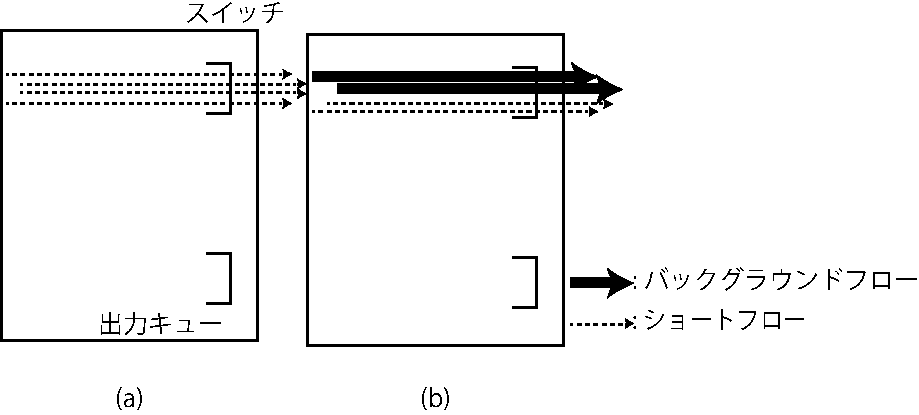
\includegraphics[autoebb, width=195pt]{./img/impairments.pdf}
    \caption{Two ways in which flows interact on a multi-ported switch
    resulting in performance problems.}
    \label{fig:impair}
    \end{center}
\end{figure}


\subsection{エンドノード - ネットワークI/O}
\label{sec:networl_io}
今日のGbE(Gigabit Ethernet)通信において, 割込み処理は大きなボトルネック要因の一つである.
例えば, 1GbEにおいて64バイトフレームの最大受信可能数は, 毎秒約150万であり, 1パケット受信する度に割り込み処理を行っていては,
CPUリソースが枯渇する.
そのため, 割込み処理の回数を抑えることが必要であるが, その分レイテンシが上がる可能性があり, 互いのトレードオフを適切に対処し高い性能を得る必要がある.
また, 今日の多くのCPUはマルチコアであり, CPUリソースを効率的に利用する事が求められている.
\subsubsection{割込み処理}
パケット受信の際のNICによるハードウェア割込みは, 即座に受信処理を行う事ができ, キューイングの遅延を小さくする事ができる.
しかし, 割込み処理が増えれば, その分オーバヘッドが大きくなり, 結果的にOSの性能が劣化する.
割込み処理を扱う代表的な仕組みとして, ポーリング, interrupt coalescingがある.

ポーリングはNICの割り込みを使わず, タイマーを使って定期的にNICの受信キューを監視することで, 割り込み負荷を軽減するソフトウェア技術である.
しかし, NICでパケットを受けてから即座に処理できない為, 遅延が発生する場合がある.
現在のLinuxカーネルにおいては, NAPIにより, 通信量が多く高負荷時のみはポーリングが作用する~\cite{NAPI}

interrupt coalescingは, 複数のパケット, あるいは一定期間待ってからをまとめて一度で割り込ませる事で,
割込み回数を減らすハードウェア技術である.
しかし, ポーリングと同様, 即座に処理できない為, 遅延が発生する場合がある.

\subsubsection{プロトコル処理}
マルチコア環境においても基本的には一つのNICの受信処理は1つのCPUでしか行えない.
そのため, ハードウェアへのアプローチとして, 1つのNICに複数の受信キューを持たせて, 受信処理をそれぞれのCPUへ分散させている, Receive
Side Scaling(RSS)がある~\cite{RSS}.
しかし, 一般に複数受信キューを持ち, RSS機能があるNICは高価である.
そのため, 一つしか受信キューを持たないNICであっても, 複数のCPUを分散させるソフトウェア技術として, RPS(Receive Packet
Sterring)がある~\cite{RPS}.
しかしRPSでは, プロトコル処理とアプリケーション処理のCPUが異なる場合が生じ, その問題を最適化したのがRFS(Receive Flow
Sterring)がある~\cite{RFS}.
これらの技術により, CPUの複数のコアをより効率良く利用する事ができる.

また, プロトコル処理やアプリケーションでの処理については, RFS等で複数のCPUへと分散させる事ができるが,
その際の割込み処理についてはオーバヘッドが生じる可能性がある.


\section{検証実験}
\label{sec:verification}
これまでの研究において報告されたMPTCPによるショートフロー性能劣化の問題~\cite{improving}を受け, その再現実験を行うことにより,
原因を解析し, 二つの要因を明らかにした~\cite{mptcp_ana}.
一つ目は, MPTCPはTCPよりも多くのトラフィックを排出し, より多くのNICインタフェースを利用する事で,
中継スイッチにおいてショートフローが利用するインタフェースと競合し, スイッチでの遅延, パケットロスが生じるということ
二つ目は, ショートフロートラフィックのバースト性の問題により, エンドノードで単一のNICに負荷が集中し, 受信処理の遅延が生じたということ
これらの結果を受け,
低レイテンシでの通信が求められるショートフローに対して, MPTCPによるバックグラウンドトラフィックが利用しているインタフェースを回避し,
比較的輻輳が起こっていない経路を適切に選ぶ事で,
単一NICへの通信負荷の問題は解消され, ショートフローのフロー完結時間(FCT)が改善できるのではないかと, 仮説を立てた.
この章では, シミュレーション, 実機での実験を用いて, その仮説の検証,
また複数のNIC, 複数の経路を利用した経路切り替えによる改善手法の効果の検証を行う.
具体的には, 中継スイッチとエンドノードへのそれぞれの単一NICの負荷について, 複数のNICを用いて分散させ, その効果を検証する.

\subsection{中継スイッチへのNIC負荷シミュレーション実験}
\subsubsection{シミュレーション環境}

ネットワークトポロジーには,
FatTreeトポロジーを部分的に抽出した2:1にオーバーサブスクリプションされたトポロジーを用いる.
図\ref{fig:topology_ns3}に, シミュレーションでトポロジーを示す.

ベンチマークトラフィックについては, 二つのペアに対してエンドノード同士の1対1通信を用いている.
一方のペアに対しては, シミュレーションを実行している間, 継続してデータ転送 (バックグラウンドトラフィック)を行う.
他方のペアに対しては, TCPによる70Kbyteのデータ転送(ショートフロー)を毎50[ms]の一様生起させ,
転送完了までにがかかった時間FCT(Flow Completion Time)を計測している.
ショートフローのルーティングに関しては, 3つのパターンを用いて中継スイッチへのインターフェースへの負荷の影響を検証する.

今回の実験にはns-3 Direct Code Execution~\cite{ns3}を用いた.
表\ref{table:testbed_ver}に再現シミュレーション環境に対する各パラメータをまとめる.
\begin{table}[h]
\begin{center}
\footnotesize
\begin{tabular}{c|c}
\hline
Parameter & Value \\ \hline \hline
Nodes & 4 \\
Link edge-edge & 200Mbps \\
Link edge-host & 100Mbps \\
RTT & 0.5ms\\
Receive buffer size & 500KB \\
\hline
\end{tabular}
\caption{シミュレーション環境パラメータ}
\label{table:testbed_ver}
\end{center}
\end{table}

\begin{figure}[h]
    \begin{center}
    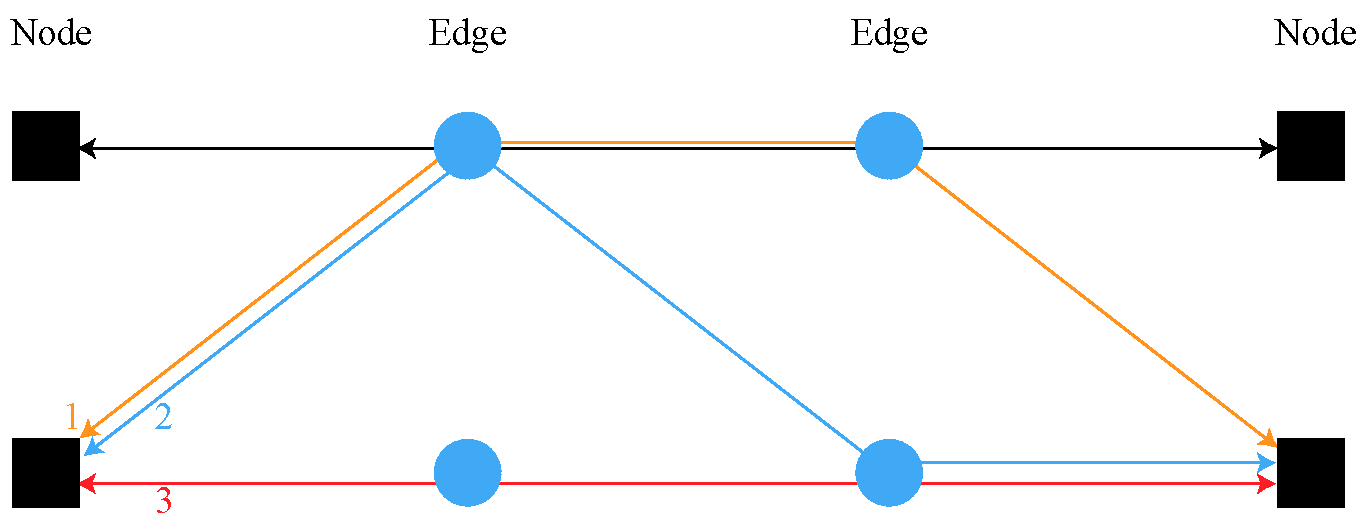
\includegraphics[autoebb, width=195pt]{./img/topology_ns3.pdf}
    \caption{中継スイッチへのNIC負荷シミュレーション実験トポロジー}
    \label{fig:topology_ns3}
    \end{center}
\end{figure}

\subsubsection{設定パラメータに対する有効性の検証}
伝搬遅延についてはRTT(Round Trip Time)として, 0.5[ms]に設定した.
これは, 一般的なデータセンター内のRTTが1[ms]以下であるためである~\cite{rtt}.

バッファサイズについては, 以下の帯域幅遅延積(BDP)の式から, 200Mbpsを最大限利用できるだけの値を設定した.
\vspace{-2mm}
\begin{eqnarray}
BDP[{\rm byte}] = 帯域幅[{\rm bps}] \times RTT \div 8
\label{cong}
\vspace{-2mm}
\end{eqnarray}

各帯域については, 4のノードを使って輻輳を引き起こす現象を再現するために, 実際のデータセンターのような広帯域のネットワークと比べ,
狭い帯域を設定した.

\subsection{検証結果}
図\ref{fig:improve}に上記の実験環境での結果として, 70KBのショートフローのFCTとバックグラウンドフローの経路利用率を示す.
この結果から, ショートフローの通信が, 中継スイッチにおいて, バックグラウンドフローと経路およびインターフェースを共有した事による影響で,
FCTの分散が大きくなっている事が分かる.
一方で, 同じスイッチは利用する事になったもののインタフェースは共有しなかったトラフィックや,
バックグラウンドフローとは独立に通信を行っていたトラフィックに対しては, 何も影響がなかった.
これは, 単一NICに対して二つのトラフィックが集中したことによる遅延,
あるいは負荷分散の影響であると考えられる.
この影響からバックグラウンドフローに対しても, スループットが下がっている事が分かる.

これらの事から, アプリケーション性能に直接影響しないBackgroung trafficが通信している中で,
低レイテンシ通信が求められているショートフローの通信をする際, 中継スイッチでの利用するインタフェースが競合する場合,
単一のNICに対しトラフィックが集中する事で, 受信処理の割込みのオーバヘッドや, プロトコル処理の遅延の影響が生じたと考えられる.
よって, 中継スイッチにおいて複数のNICに対し, トラフィックを分散させる事は, レイテンシ志向のショートフローに対しても,
スループット志向のバックグラウンドフローに対しても有効であるといえる.

\begin{figure}[h]
    \begin{center}
    \includegraphics[autoebb, width=195pt]{./img/switch_verif.pdf}
    \caption{70kbベンチマークトラフィックに対するフロー完結時間とリンク利用率}
    \label{fig:improve}
    \end{center}
\end{figure}

\subsection{エンドノードへのNIC負荷実機実験}
\subsubsection{実験環境}
複数のNICを用いた負荷分散手法のバースト性のあるショートフロートラフィックに対する影響を検証する.
ネットワークトポロジーには,
図\ref{fig:fattree_ver}に示すように, 二つのNICを持った二つエンドノード同士をL2スイッチを介してそれぞれのNIC毎に接続した.
ルーティングに関しては, それぞれの対をなすNIC同士が通信を行う.
ベンチマークトラフィックについては, エンドノード同士の1対1通信を用い, ショートフローとバックグラウンドフローを通信させる.
バックグラウンドフローについては,
ショートフローが通信しているNICペアと同じものを使って共有して通信させるパターンとショートフローが通信しているNICペアとは異なるペアのNICを用いて通信を行うパターンの2パターンについて検証する.
ショートフローは, TCPによる10Kbyteのデータ転送を毎10ms, 30フローを同時に一様生起させ, 転送完了までにがかかった時間FCT(Flow
Completion Time)を計測している.
バックグラウンドトラフィックは, シミュレーションを実行している間, 継続してデータ転送を行う.

図\ref{fig:fattree_rep}に, シミュレーションで用いたトポロジーを示す.
表\ref{table:experiment_ver}に実験環境に対する各パラメータをまとめる.
\begin{table}[h]
\begin{center}
\footnotesize
\begin{tabular}{c|c}
\hline
Parameter & Value \\ \hline \hline
OS & Linux 3.13.0 \\
リンク経路 & 1Gbps \\
RTT & 0.2ms\\
MAX receive buffer size & 6144KB \\
MAX ring buffer & 4096 \\
\hline
\end{tabular}
\caption{実験環境パラメータ}
\label{table:experiment_ver}
\end{center}
\end{table}

\begin{figure}[h]
    \begin{center}
    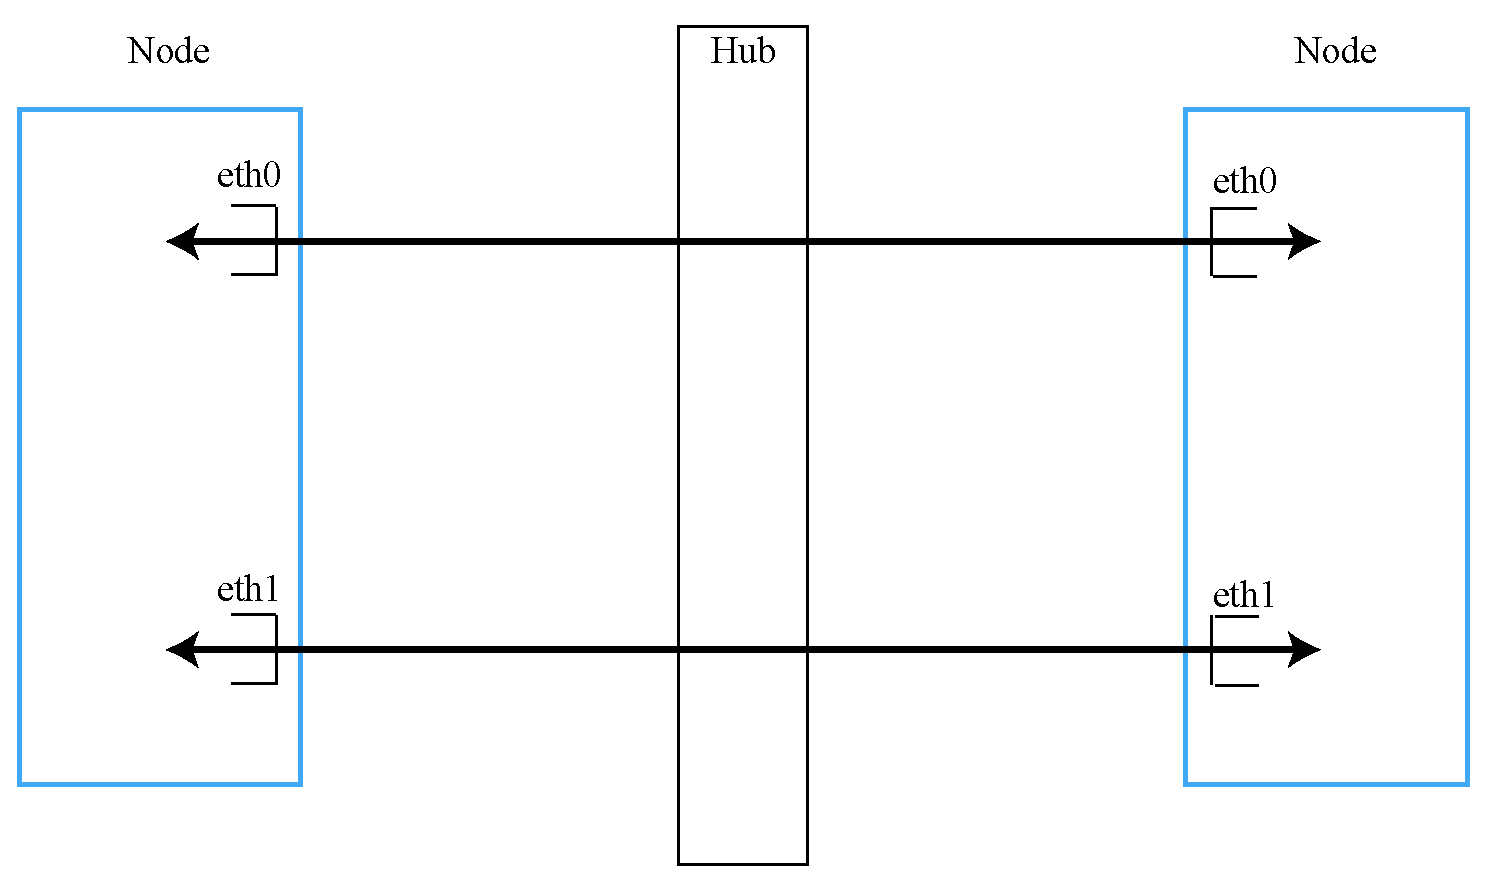
\includegraphics[autoebb, width=195pt]{./img/topology_real.pdf}
    \caption{エンドノードへのNIC負荷実機実験トポロジー}
    \label{fig:topology_real}
    \end{center}
\end{figure}

\subsection{検証結果}
図\ref{fig:real_exp0}, 図\ref{fig:real_exp1}に上記の実験環境での結果として,
10KBのショートフローのFCTとそれぞれの経路の利用率を示す.
この結果から, ショートフローの通信が, エンドノード間通信において, バックグラウンドフローと経路およびインターフェースを共有した事による影響で,
FCTの分散が大きくなっている事が分かる.
一方で, 経路, インタフェースは競合しなかったものの, バックグラウンドフローとショートフローが同時に通信を行ったことで,
FCT下位25\%のフローについては遅延が生じ, 分散が大きくなった.
これは, 単一NICに対して二つのトラフィックが集中したことによる負荷分散の効果が得られたが, プロトコル処理以降の部分で,
複数のフローが同時に通信を行った事に対するオーバヘッドが生じたと考えられる.
またバックグラウンドフローに着目すると, インターフェースを共有した場合においては,
ショートフローだけでなくバックグラウンドフローにも遅延が生じ, スループットが低下している.

これらの事から, アプリケーション性能に直接影響しないBackgroung trafficが通信している中で,
バースト性のあるショートフロートラフィックの通信をする際, エンドノードに対して, 利用するインタフェースが競合する場合,
単一のNICに対しトラフィックが集中する事で, 受信処理の割込みのオーバヘッドや, プロトコル処理の遅延の影響があると考えられる.
よって, エンドノードにおいて複数のNICに対し, トラフィックを分散させる事は, バースト性のあるショートフローに対しても,
スループット志向のバックグラウンドフローに対しても有効であるといえる.

\begin{figure}[h]
    \begin{center}
    \includegraphics[autoebb, width=195pt]{./img/real_eth0.pdf}
    \caption{10kbベンチマークトラフィックに対するフロー完結時間とリンク利用率[eth0]}
    \label{fig:real_exp0}
    \end{center}
\end{figure}

\begin{figure}[h]
    \begin{center}
    \includegraphics[autoebb, width=195pt]{./img/real_eth1.pdf}
    \caption{10kbベンチマークトラフィックに対するフロー完結時間とリンク利用率[eth1]}
    \label{fig:real_exp1}
    \end{center}
\end{figure}

\subsection{考察}
\label{sec:analysis}
これらの解析結果から, エンドノード, スイッチに対する機能障害が引き起こる要因について述べ, 今後の改善手法の検討を行う.\\
大量の計算機資源をいかに効率的に利用するか, という課題を今日のデータセンターは抱えており,
Hadoopのような並列分散処理アプリケーションを用いる事が一般的である.
今の並列分散処理システムがpartition-aggrigation構造である以上, 管理ノードや多段のクラスター構成であればアグリゲーターノードに対して, 処理ノードからのトラフィックが集中する問題は発生する.
その結果, {\bf Queue buildup}や{\bf Incast}のような単一NICへの負荷集中の問題が中継スイッチやエンドノードに対して生じ, 並列分散処理の性能が劣化する.

こうした遅延の影響を軽減する為には, 混雑時の通信量を抑える制御を行う, あるいは混雑時にも空いているリソースを効率良く利用する事が必要である.
MPTCPのような, 既存の計算機資源に対して複数NICを刺して性能向上を目指すことで, 複数のフローからデータを受信する際に異なる物理ポートを利用する事で,
マルチコアを持つCPUの効率的な利用につなげられると期待している.
すなわち, 複数のNICに対して通信を分散させるように, トラフィックを制御する事で,
例えばレイテンシ志向なショートフローとスループット志向なバックグラウンドフローのような役割の異なるトラフィックを共存させ,
最適な通信の実現が可能であることを本論文では示した.
そのような複数のNICが介在するネットワークの中で, トラフィックをどのように制御するかという点については,
スイッチやエンドノードのOSスタック等のどこで制御をするか, またどのようなアルゴリズムでそれを実現するかという事を検討する必要がある.


% \subsubsection{Background traffic}
% Background
% trafficに対する評価として全12の処理ノードへ平均500[ms]のポアソン生起でフローサイズ1[KB]$\sim$1[MB]のトラフィックを同時に発生させた状態で,
% 同時に12の処理ノードへ平均500[ms]のポアソン生起でトラフィックを発生させ, 各経路のスループットを計測した.
% その結果を図\ref{fig:background}に示す.
%
% この結果から, MPTCPはBackground trafficに対し, TCPよりも性能向上が見られることが分かる.
% これは, MPTCPのロードバランスと複数経路を使って並行的にデータを送信したことによるものである.
%
% \begin{figure}[h]
%     \begin{center}
%     \includegraphics[autoebb, width=180pt]{./img/back.pdf}
%     \caption{Throughput of background traffic}
%     \label{fig:background}
%     \end{center}
% \end{figure}
% \hspace{1cm}

\section{あとがき}
\label{sec:conclude}
本論文では, データセンターにおけるショートフロー遅延の問題を解決する為に, 二つの検証を行った.

一つは, 実環境の並列分散処理アプリケーションが稼働しているクラスターPCを用いて, 実トラフィックの観測, 解析を行った.
クラスターPCがジョブを実行していない定常状態時と並列分散処理を実行している時の二種類のトラフィックを解析することで,
並列分散処理アプリケーションが生成するトラフィックパターンの特徴および, 汎用的なネットワーク機器を用いた低コストなデータセンターにおける要求案件を検証した.
そして, ショートフロー遅延が生じる状況と既存のネットワーク設計の背景について, ボトルネックとなりうるネットワーク環境を検討し, その原因を示した.

二つ目は, MPTCPを用いたデータセンターネットワークモデルにおける, 複数のNIC, 複数の経路を利用した経路切り替えによる改善手法を提案する.
これは, 複数の経路を利用しスイッチやエンドノードの持つ複数のNICへと負荷を分散させることで, 単一のNICに負荷が集中することによる,
キューイングやプロトコル処理の遅延を抑える事ができる, という仮定に基づき, 提案する手法である.
この手法により, 並列分散処理におけるショートフローのような, 低レイテンシが求められる通信においては, 他のフローの影響を受けずにすぐに割込み処理が行われ, 受信処理のCPU負荷の分散を期待し, その効果をシミュレーション, 実環境での実験を用いて検証した.
そして今後の課題として, 経路切り替えのアルゴリズム検討する.


本論文では, サイズが大きく長時間通信を行うバックグラウンドトラフィックとサイズが小さくフロー完結時間を短く抑えたいショートフローが混在する状況において, フローサイズの小さいトラフィックに対しては,
従来のTCPよりもデータ転送に時間がかかるという問題に対して, 改善手法の効果を検証した.
また, 実環境の並列分散処理アプリケーションが稼働しているクラスターPCを用いて,
ジョブを実行していない定常状態時と並列分散処理を実行している時の二種類のトラフィックを解析を行い, 単一のNICに対して通信負荷が集中する問題がある事を示し,
通信経路を切り替える事により, 複数のNICに対し負荷分散するという改善手法を提案した.
この改善手法により, 他のフローの影響を受けずにすぐに割込み処理が行われ, レイテンシ志向なショートフローへの受信処理の遅延を軽減する事ができた.
また, スループット志向であるバックグラウンドフローに対しても, 通信性能を向上させる事ができた.

今後はネットワークの通信状況を考慮しながら, 通信経路を切り替えるアルゴリズムの検討を行う.
%\bibliographystyle{sieicej}
%\bibliography{myrefs}
\begin{spacing}{0.7}
\footnotesize{
\begin{thebibliography}{99}% 文献数が10未満の時 {9}
\bibitem{IBM_rep}{日本アイ・ビー・エム株式会社. IBM 第1章
大容量データのバックアップ,
\url{http://www-06.ibm.com/systems/jp/storage/column/backup/01.html}}
\bibitem{amazon}{Jim Liddle. Amazon found every 100ms of latency cost them 1\%
in sales, August 2008.
\url{http://blog.gigaspaces.com/amazon-found-every-100ms-of-latency-cost}

\url{-them-1-in-sales/}}

\bibitem{customer_impact}{R. Kohavi et al. Practical Guide to Controlled
Experiments on theWeb: Listen to Your Customers not to the HiPPO. KDD, 2007.}
\bibitem{requirement}{J. Hamilton. On designing and deploying Internet-scale
services. In USENIX LISA, 2007.}
\bibitem{presto}{Facebook. Presto: Interacting with petabytes
of data at Facebook,
\url{https://www.facebook.com/notes/facebook-engineering/presto-interacting-with-petabytes-of-data}

\url{-at-facebook/10151786197628920}}
\bibitem{mapreduce}{Dean, Jeffrey, and Sanjay
Ghemawat. "MapReduce: simplified data processing on large clusters." Communications of the ACM 51.1 (2008): 107-113.} \bibitem{dryad}{Isard, Michael, et al. "Dryad: distributed data-parallel
programs from sequential building blocks." ACM SIGOPS Operating Systems Review 41.3 (2007): 59-72.}
\bibitem{fattree}{Al-Fares, Mohammad, Alexander Loukissas, and Amin Vahdat. "A
scalable, commodity data center network architecture." ACM SIGCOMM Computer Communication Review. Vol. 38. No. 4. ACM, 2008.}
\bibitem{bcube}{Guo, Chuanxiong, et al. "BCube: a high performance,
server-centric network architecture for modular data centers." ACM SIGCOMM Computer Communication Review 39.4 (2009): 63-74.}
\bibitem{vl2}{Greenberg, Albert, et al. "VL2: a scalable and flexible data
center network." ACM SIGCOMM Computer Communication Review. Vol. 39. No. 4. ACM, 2009.}
\bibitem{dctcp}{Alizadeh, Mohammad, et al. "Data center tcp (dctcp)." ACM SIGCOMM Computer Communication Review 40.4 (2010): 63-74.}
\bibitem{improving}{Raiciu, Costin, et al. "Improving datacenter performance and
robustness with multipath TCP." ACM SIGCOMM Computer Communication Review. Vol. 41. No. 4. ACM, 2011.}
\bibitem{detail}{Zats, David, et al. "DeTail: Reducing the flow completion time
tail in datacenter networks." ACM SIGCOMM Computer Communication Review 42.4 (2012): 139-150.}
\bibitem{p_fab}{Alizadeh, Mohammad, et al. "pfabric: Minimal near-optimal datacenter transport." Proceedings of the ACM SIGCOMM 2013 conference on SIGCOMM. ACM, 2013.}
\bibitem{click}{Kohler, Eddie, et al. "The Click modular router." ACM
Transactions on Computer Systems (TOCS) 18.3 (2000): 263-297.}
\bibitem{mptcp}{Ford, Alan, et al. TCP Extensions for Multipath Operation with
Multiple Addresses: draft-ietf-mptcp-multiaddressed-03. No. Internet draft (draft-ietf-mptcp-multiaddressed-07). Roke Manor, 2011.}
\bibitem{cong}{Raiciu, C., M. Handley, and D. Wischik. "Coupled congestion
control for multipath transport protocols." draft-ietf-mptcp-congestion-01 (work in progress) (2011).}
\bibitem{ns3}{Inria「DCE - GETTING STARTED Direct Code Execution」
\url{http://www.nsnam.org/~thehajime/ns-3-dce-doc/getting-started.html}}
\bibitem{traffic}{Benson, Theophilus, Aditya Akella, and David A. Maltz.
"Network traffic characteristics of data centers in the wild." Proceedings of the 10th ACM SIGCOMM conference on Internet measurement. ACM, 2010.}
\bibitem{NAPI}{J. Salim, When NAPI Comes to Town, Proceedings of Linux 2005
Conference, UK, August 2005.}
\bibitem{RSS}{Microsoft corporation. scalable networking with rss, 2005.}
\bibitem{RFS}{Herbert, T. rfs: receive flow steering, september 2010.
http://lwn.net/Articles/381955/.}
\bibitem{RPS}{Herbert, T. rps: receive packet steering, september 2010.
http://lwn.net/Articles/361440/.}
\bibitem{mptcp_linux}{ip networking lab「MultiPath
TCP - Linux Kernel implementation」\url{http://mptcp.info.ucl.ac.be/}}
\bibitem{rtt}{Vasudevan, Vijay, et al. "Safe and effective fine-grained TCP
retransmissions for datacenter communication." ACM SIGCOMM Computer Communication Review. Vol. 39. No. 4. ACM, 2009.}
\bibitem{mptcp_ana}{藤居 翔吾, 田崎 創, 関谷 勇司, "MultiPath TCP
適用時のデータセンターネットワークでのフローサイズが与える影響に関する一考察", 電子情報通信学会, 信学技法, vol. 113, no. 364,
IA2013-65, pp. 47-52, 2013.}
\bibitem{flexible}{P. Agarwal, B. Kwan, and L. Ashvin. Flexible buffer allocation entities for
traffic aggregate containment. US Patent 20090207848, August 2009.}
\bibitem{synchro}{S. Floyd and V. Jacobson. The synchronization of periodic routing messages.
IEEE/ACM ToN, 1994.}
\bibitem{balia}{A. Walid, et al. Balanced Linked Adaptation Congestion Control
Algorithm for MPTCP draft-walid-mptcp-congestion-control-00, 2014.}

\end{thebibliography}
}
\end{spacing}


\end{document}